\documentclass[a4paper,12pt]{article}
\usepackage[utf8]{inputenc}
\usepackage[german]{babel}
\usepackage{amsmath}
\usepackage{amssymb}
\usepackage{amsthm}
\usepackage{geometry}
\usepackage{graphicx}
\usepackage[hidelinks]{hyperref}
\usepackage{listings}
\usepackage{xcolor}
\usepackage{enumitem}
\usepackage{microtype}

\geometry{margin=2.5cm}
\sloppy

\theoremstyle{definition}
\newtheorem{definition}{Definition}
\newtheorem{beispiel}{Beispiel}
\newtheorem{satz}{Satz}
\newtheorem{lemma}{Lemma}
\newtheorem{bemerkung}{Bemerkung}
\newtheorem{korollar}{Korollar}

\setlist[itemize,1]{label=--}

% ---------- Farben ----------
\definecolor{mainblue}{RGB}{25, 70, 140}
\definecolor{accentred}{RGB}{180, 50, 30}
\definecolor{lightgray}{RGB}{245, 245, 248}
\definecolor{darkgray}{RGB}{60, 60, 70}
\definecolor{darkgreen}{RGB}{30, 100, 50}

\hypersetup{
	colorlinks=true,
	linkcolor=mainblue,
	citecolor=accentred,
	urlcolor=mainblue
}

\lstset{
	basicstyle=\ttfamily\small,
	keywordstyle=\color{blue},
	commentstyle=\color{gray},
	stringstyle=\color{red},
	numbers=left,
	numberstyle=\tiny,
	breaklines=true,
	frame=single,
	literate=%
	{Ö}{{\"O}}1
	{Ä}{{\"A}}1
	{Ü}{{\"U}}1
	{ß}{{\ss}}1
	{ü}{{\"u}}1
	{ä}{{\"a}}1
	{ö}{{\"o}}1
	{Σ}{{$\Sigma$}}1
	{→}{{$\rightarrow$}}1
	{⊆}{{$\subseteq$}}1
	{⊇}{{$\supseteq$}}1
	{≥}{{$\geq$}}1
}

\title{Redundanzsicherheit: Eine Vereinheitlichung von Funktionaler Sicherheit\\ und Cyber Security}
\author{Stephan Epp}
\date{30. Juni 2026}

\begin{document}

\maketitle

\tableofcontents
\newpage

\section{Einführung}

In der Automotive- und Embedded-Praxis werden Funktionale Sicherheit (Safety, z.\,B. nach ISO~26262) und Cyber Security üblicherweise als zwei getrennte Disziplinen mit getrennten Zielsystemen behandelt: Safety schützt die Funktion vor zufälligen oder systematischen Fehlern, Security schützt das System vor vorsätzlichen Angriffen. Diese Trennung ist organisatorisch bequem, aber technisch inkonsequent. In dieser Arbeit wird formal gezeigt, dass es Systemzustände gibt, in denen ein Safety-Mechanismus die korrekte Funktion sicherstellt, obwohl ein Cyberangriff das Steuergerät bereits erfolgreich manipuliert hat. Die Sicherheit der Funktion wird in diesem Fall ausschließlich durch \emph{Redundanz} hergestellt -- unabhängig davon, ob die Störungsursache zufällig (Safety) oder vorsätzlich (Security) war.

\subsection{Problemstellung}

Gegeben sei ein Steuergerät, das eine Funktion $f$ über $n$ redundante, voneinander unabhängige Kanäle (Recheneinheiten, Sensoren, Software-Instanzen) realisiert. Jeder Kanal kann unabhängig kompromittiert werden -- durch einen Hardwarefehler (klassische Safety-Perspektive) oder durch einen gezielten Cyberangriff (klassische Security-Perspektive). Eine Entscheidungsinstanz (Voter) bestimmt aus den $n$ Kanalausgaben das resultierende Funktionsergebnis.

\textbf{Zentrale Beobachtung:} Die klassische Trennung von Safety und Security beantwortet zwei verschiedene Fragen:
\begin{itemize}
	\item \textbf{Safety-Frage:} Ist die Funktionsausgabe korrekt?
	\item \textbf{Security-Frage:} Ist die Integrität \emph{aller} Kanäle gewahrt?
\end{itemize}

Diese beiden Fragen sind \emph{nicht äquivalent}. Es existieren Zustände, in denen die Safety-Frage mit „Ja'' und die Security-Frage gleichzeitig mit „Nein'' zu beantworten ist. Genau dieser Widerspruch wird in dieser Arbeit formal modelliert, bewiesen und quantifiziert.

\textbf{Ziel:} Entwicklung eines einheitlichen, redundanzbasierten Sicherheitsbegriffs (Redundanzsicherheit), der Safety und Security als Spezialfälle eines gemeinsamen Modells auffasst, anstatt sie als unabhängige Eigenschaften zu behandeln.

\subsection{Motivation}

Die Praxis der funktionalen Sicherheit verwendet Redundanz (z.\,B. Triple Modular Redundancy, Lockstep-Prozessoren, diversitäre Software-Pfade) explizit zur Fehlertoleranz gegenüber zufälligen Fehlern. Die Praxis der Cyber Security verwendet Mechanismen wie Signaturprüfung, Secure Boot und Intrusion Detection zur Verhinderung vorsätzlicher Manipulation. Beide Disziplinen nutzen jedoch im Kern dasselbe strukturelle Prinzip: \emph{Ein einzelner kompromittierter Bestandteil darf das Gesamtergebnis nicht bestimmen.} Diese Arbeit zeigt, dass dieses Prinzip -- Redundanz mit Mehrheitsentscheidung -- die gemeinsame, hinreichende Bedingung für funktionale Korrektheit ist, gleich welcher Natur die zugrunde liegende Störung ist. Die Unterscheidung „Safety vs. Security'' beschreibt lediglich die \emph{Ursache} der Kanalkompromittierung, nicht aber die \emph{Wirkung} auf das Gesamtsystem.

\section{Grundlagen}

\subsection{Definitionen}

\begin{definition}[Kanal]
	Ein Kanal $c_i$, $i \in \{0,\ldots,n-1\}$, ist eine unabhängige Realisierung einer Funktion $f: X \to Y$, die für eine Eingabe $x \in X$ eine Ausgabe $c_i(x) \in Y$ liefert.
\end{definition}

\begin{definition}[Kompromittierung]
	Ein Kanal $c_i$ heißt \emph{kompromittiert} für Eingabe $x$, wenn $c_i(x) \neq f(x)$ gilt, wobei $f(x)$ die spezifikationsgemäße korrekte Ausgabe bezeichnet. Die Ursache der Kompromittierung -- zufälliger Hardwarefehler (Safety-Ereignis) oder vorsätzlicher Eingriff (Security-Ereignis) -- bleibt für diese Definition irrelevant.
\end{definition}

\begin{definition}[Kompromittierungsindikator]
	Für Kanal $c_i$ und Eingabe $x$ sei
	\[
	K_i(x) = \begin{cases}
		1 & \text{falls } c_i(x) \neq f(x) \text{ (kompromittiert)} \\
		0 & \text{sonst (intakt)}
	\end{cases}
	\]
	Wir modellieren $K_i(x)$ für ein festes $x$ als Bernoulli-verteilte Zufallsvariable mit Parameter $p \in [0,1]$, $K_i(x) \sim \mathrm{Bernoulli}(p)$, unabhängig über $i$ (Unabhängigkeitsannahme A1).
\end{definition}

\begin{definition}[Mehrheits-Voter]
	Der Mehrheits-Voter $V_n: Y^n \to Y$ liefert für $n$ Kanalausgaben $(y_0,\ldots,y_{n-1})$ denjenigen Wert $y^\ast$, der unter den $n$ Werten am häufigsten auftritt. Für ungerades $n$ ist $y^\ast$ eindeutig bestimmt, falls mehr als $\lfloor n/2 \rfloor$ Kanäle übereinstimmen.
\end{definition}

\begin{definition}[Safety-Prädikat]
	Das Safety-Prädikat $S(x)$ ist wahr genau dann, wenn die Voter-Ausgabe korrekt ist:
	\[
	S(x) :\Leftrightarrow V_n(c_0(x),\ldots,c_{n-1}(x)) = f(x).
	\]
\end{definition}

\begin{definition}[Security-Prädikat]
	Das Security-Prädikat $T(x)$ ist wahr genau dann, wenn \emph{kein} Kanal kompromittiert ist:
	\[
	T(x) :\Leftrightarrow \sum_{i=0}^{n-1} K_i(x) = 0.
	\]
\end{definition}

\subsection{Grundidee}

Die Kernidee der Redundanzsicherheit besteht darin, dass $S(x)$ eine \emph{schwächere} Bedingung als $T(x)$ ist: $S(x)$ verlangt lediglich, dass eine Mehrheit der Kanäle korrekt ist, während $T(x)$ verlangt, dass \emph{alle} Kanäle korrekt sind. Da bei Mehrheitsentscheidung bereits eine knappe Mehrheit genügt, kann $S(x)$ wahr sein, obwohl $T(x)$ falsch ist -- dies ist der formale Kern des in der Einleitung beschriebenen Phänomens.

\section{Formale Ergebnisse}

\subsection{Logische Beziehung zwischen Safety und Security}

\begin{satz}[Echte Implikation]
	\label{satz:implikation}
	Für jeden Mehrheits-Voter $V_n$ mit $n \geq 3$ und jede Eingabe $x$ gilt:
	\[
	T(x) \;\Rightarrow\; S(x), \qquad \text{aber} \qquad S(x) \not\Rightarrow T(x).
	\]
\end{satz}

\begin{proof}
	\textbf{Richtung $T(x) \Rightarrow S(x)$:} Ist $T(x)$ wahr, so gilt $K_i(x) = 0$ für alle $i$, also $c_i(x) = f(x)$ für alle $i$. Damit stimmen alle $n$ Kanäle überein, und der Mehrheits-Voter liefert trivial $V_n(c_0(x),\ldots,c_{n-1}(x)) = f(x)$, also $S(x)$.

	\textbf{Gegenbeispiel zu $S(x) \Rightarrow T(x)$:} Sei $n = 3$. Betrachte $c_0(x) = c_1(x) = f(x)$ und $c_2(x) \neq f(x)$ (Kanal 2 kompromittiert, etwa durch einen erfolgreichen Cyberangriff auf genau diesen Kanal). Die Mehrheit von zwei der drei Kanäle liefert $f(x)$, also gilt $V_3(c_0(x),c_1(x),c_2(x)) = f(x)$ und damit $S(x)$. Gleichzeitig gilt $K_2(x) = 1$, also $\sum_i K_i(x) = 1 \neq 0$, somit ist $T(x)$ falsch. Damit ist $S(x) \wedge \neg T(x)$ erfüllbar, die Rückrichtung ist also widerlegt. \qedhere
\end{proof}

\begin{korollar}[Inkonsequenz der getrennten Betrachtung]
	\label{kor:inkonsequenz}
	Die Aussage „das System ist sicher'' ist unter getrennter Safety-/Security-Bewertung nicht wohldefiniert: Es existieren Zustände mit $S(x) = 1$ und $T(x) = 0$, in denen ein reines Safety-Audit das System als sicher klassifiziert, während ein reines Security-Audit denselben Zustand als kompromittiert klassifiziert. Beide Aussagen sind über denselben Systemzustand korrekt und widersprechen sich dennoch in der Bewertung „sicher/unsicher''.
\end{korollar}

\begin{proof}
	Folgt unmittelbar aus Satz~\ref{satz:implikation}: Im dort konstruierten Zustand ist $S(x)=1$ (Safety-Bewertung: sicher) und $T(x)=0$ (Security-Bewertung: unsicher) gleichzeitig wahr für denselben $x$. \qedhere
\end{proof}

\subsection{Quantifizierung der Divergenz}

\begin{satz}[Wahrscheinlichkeit korrekter Funktion]
	\label{satz:pkorrekt}
	Sei $n$ ungerade, $K_i(x) \sim \mathrm{Bernoulli}(p)$ i.i.d.\ für $i=0,\ldots,n-1$ (Annahme A1), und die Kompromittierung jedes Kanals führe stets zu einer von $f(x)$ verschiedenen Ausgabe (Annahme A2: keine zufällige Kompromittierung trifft zufällig wieder $f(x)$). Dann gilt für die Wahrscheinlichkeit korrekter Funktionsausgabe
	\[
	P_{\mathrm{Safety}}(n,p) := \Pr[S(x)] = \sum_{k=0}^{\lfloor (n-1)/2 \rfloor} \binom{n}{k} p^k (1-p)^{n-k}.
	\]
\end{satz}

\begin{proof}
	Unter A2 stimmen genau die intakten Kanäle in ihrem Wert $f(x)$ überein; kompromittierte Kanäle liefern (im ungünstigsten, aber unter A2 zulässigen Fall) jeweils einen von $f(x)$ verschiedenen, untereinander nicht notwendig übereinstimmenden Wert. Der Mehrheits-Voter liefert genau dann $f(x)$, wenn die Anzahl $K := \sum_i K_i(x)$ kompromittierter Kanäle kleiner oder gleich $\lfloor (n-1)/2 \rfloor$ ist, denn dann bilden die intakten Kanäle mit $n-K \geq \lceil (n+1)/2 \rceil$ Stimmen die größte Gruppe, selbst wenn alle kompromittierten Kanäle (im ungünstigsten Fall) auf einen einzigen falschen Wert kollabieren. $K$ ist nach A1 binomialverteilt mit Parametern $(n,p)$, woraus die Behauptung durch Aufsummieren der Wahrscheinlichkeitsmasse $\Pr[K \leq \lfloor (n-1)/2\rfloor]$ folgt. \qedhere
\end{proof}

\begin{satz}[Wahrscheinlichkeit vollständiger Integrität]
	\label{satz:psecure}
	Unter denselben Annahmen wie in Satz~\ref{satz:pkorrekt} gilt
	\[
	P_{\mathrm{Security}}(n,p) := \Pr[T(x)] = (1-p)^n.
	\]
\end{satz}

\begin{proof}
	$T(x)$ ist genau dann wahr, wenn alle $n$ Indikatoren $K_i(x)$ gleich $0$ sind. Da diese nach A1 unabhängig und identisch $\mathrm{Bernoulli}(p)$-verteilt sind, gilt $\Pr[K_0(x)=0 \wedge \cdots \wedge K_{n-1}(x)=0] = \prod_{i=0}^{n-1}\Pr[K_i(x)=0] = (1-p)^n$. \qedhere
\end{proof}

\begin{satz}[Strikte Divergenz für $n \geq 3$]
	\label{satz:divergenz}
	Für jedes ungerade $n \geq 3$ und jedes $p \in (0,1)$ gilt
	\[
	P_{\mathrm{Safety}}(n,p) > P_{\mathrm{Security}}(n,p).
	\]
\end{satz}

\begin{proof}
	Es gilt $P_{\mathrm{Security}}(n,p) = (1-p)^n = \binom{n}{0}p^0(1-p)^{n-0}$, also genau der $k=0$-Summand von $P_{\mathrm{Safety}}(n,p)$ aus Satz~\ref{satz:pkorrekt}. Für $n \geq 3$ ist $\lfloor (n-1)/2 \rfloor \geq 1$, sodass die Summe in $P_{\mathrm{Safety}}(n,p)$ mindestens den zusätzlichen, für $p \in (0,1)$ strikt positiven Summanden $\binom{n}{1}p^1(1-p)^{n-1} > 0$ enthält. Da alle Summanden der Binomialverteilung nichtnegativ sind, folgt
	\begin{align*}
	P_{\mathrm{Safety}}(n,p) &= (1-p)^n + \binom{n}{1}p(1-p)^{n-1} + \sum_{k=2}^{\lfloor (n-1)/2\rfloor} \binom{n}{k}p^k(1-p)^{n-k} \\
	&> (1-p)^n = P_{\mathrm{Security}}(n,p). \qedhere
	\end{align*}
\end{proof}

\begin{bemerkung}
	Satz~\ref{satz:divergenz} zeigt, dass die Divergenz zwischen Safety- und Security-Garantie kein Randphänomen, sondern für jeden nichttrivialen redundanten Mehrheits-Voter ($n\geq 3$) und jede positive Kompromittierungswahrscheinlichkeit \emph{strukturell unvermeidlich} ist. Abbildung~\ref{fig:divergenz} veranschaulicht diese Divergenz für $n=5$.
\end{bemerkung}

\subsection{Monotonie und Grenzverhalten}

\begin{lemma}[Monotonie in $n$]
	\label{lem:monotonie}
	Für festes $p \in (0, 0.5)$ ist $P_{\mathrm{Safety}}(n,p)$ streng monoton wachsend in $n$ über die ungeraden $n \geq 1$.
\end{lemma}

\begin{proof}
	Der Übergang von $n$ auf $n+2$ Kanälen (Hinzufügen eines symmetrischen Kanalpaares zur Erhaltung der Eindeutigkeit der Mehrheit) ist ein Standardresultat der Theorie robuster Mehrheitsentscheidungen (vgl. Condorcet-Jury-Theorem, \cite{condorcet1785}): Für $p < 0.5$ erhöht ein zusätzliches, unabhängiges Paar korrekter-im-Erwartungswert-Kanäle die Wahrscheinlichkeit, dass die Mehrheit korrekt entscheidet, da der Erwartungswert der Mehrheitsstimmen weiter von der Entscheidungsschwelle $n/2$ wegrückt. Formal folgt dies aus der strikten Monotonie der regularisierten unvollständigen Betafunktion $I_{1-p}(n-k,k+1)$ in $n$ für festes $k/n < 1-p$, einer Standardidentität zwischen Binomialsummen und der Betafunktion. \qedhere
\end{proof}

\begin{lemma}[Grenzverhalten]
	\label{lem:grenzwert}
	Für festes $p \in (0,0.5)$ gilt $\lim_{n\to\infty} P_{\mathrm{Safety}}(n,p) = 1$ und $\lim_{n\to\infty} P_{\mathrm{Security}}(n,p) = 0$.
\end{lemma}

\begin{proof}
	Für $P_{\mathrm{Security}}(n,p) = (1-p)^n$ mit $p>0$ folgt $(1-p)^n \to 0$ für $n \to \infty$ direkt aus $0 < 1-p < 1$.

	Für $P_{\mathrm{Safety}}(n,p)$ betrachte den Anteil $K/n$ kompromittierter Kanäle. Nach dem schwachen Gesetz der großen Zahlen konvergiert $K/n$ für $n\to\infty$ in Wahrscheinlichkeit gegen $p$. Da $p < 0.5$, liegt der Grenzwert $p$ unterhalb der Mehrheitsschwelle $1/2$, sodass $\Pr[K/n \leq \lfloor (n-1)/2\rfloor/n] \to 1$ für $n \to \infty$ gilt (Anwendung der Chernoff-Schranke liefert zusätzlich exponentiellen Abfall der Restwahrscheinlichkeit: $\Pr[K > n/2] \leq e^{-n \cdot D(0.5 \| p)}$ mit Kullback-Leibler-Divergenz $D(0.5\|p) > 0$ für $p \neq 0.5$). Damit folgt $P_{\mathrm{Safety}}(n,p) \to 1$. \qedhere
\end{proof}

\begin{bemerkung}
	Lemma~\ref{lem:grenzwert} liefert die formale Pointe der Arbeit: Mit wachsendem Redundanzgrad $n$ konvergiert die Safety-Garantie gegen Gewissheit, während die Security-Garantie (vollständige Integrität aller Kanäle) gegen Null konvergiert. Mehr Redundanz macht das System also \emph{sicherer im Sinne der Funktion} und gleichzeitig \emph{garantiert unsicherer im Sinne vollständiger Integrität}. Dies ist kein Widerspruch, sondern der formale Beleg dafür, dass „Security'' im Sinne vollständiger Integrität aller Komponenten das falsche Zielprädikat für ein redundantes System ist -- das relevante Zielprädikat ist $S(x)$, die Redundanzsicherheit.
\end{bemerkung}

\subsection{Mindestredundanzgrad}

\begin{satz}[Hinreichender Redundanzgrad]
	\label{satz:minimalradundanz}
	Sei $p \in (0,0.5)$ und $\delta \in (0,1)$ ein Zielwert für die maximal tolerierte Ausfallwahrscheinlichkeit $1 - P_{\mathrm{Safety}}(n,p)$. Dann genügt
	\[
	n \;\geq\; \frac{2\ln(1/\delta)}{D(0.5\,\|\,p)}
	\]
	mit Kullback-Leibler-Divergenz $D(0.5\|p) = 0.5\ln\frac{0.5}{p} + 0.5\ln\frac{0.5}{1-p}$, um $1 - P_{\mathrm{Safety}}(n,p) \leq \delta$ für ungerades $n$ sicherzustellen.
\end{satz}

\begin{proof}
	Nach der Chernoff-Schranke für Binomialverteilungen gilt für $K \sim \mathrm{Bin}(n,p)$ mit $p < 0.5$:
	\[
	\Pr[K \geq n/2] \;\leq\; e^{-n \cdot D(0.5\|p)}.
	\]
	Da $1 - P_{\mathrm{Safety}}(n,p) = \Pr[K > \lfloor (n-1)/2\rfloor] \leq \Pr[K \geq n/2]$ für ungerades $n$, genügt $e^{-n\cdot D(0.5\|p)} \leq \delta$, äquivalent $n \geq \ln(1/\delta)/D(0.5\|p)$. Der Faktor $2$ im Zähler der Behauptung ist eine konservative Sicherheitsmarge, die in der Praxis numerische Rundung beim nächsten ungeraden $n$ sowie die Differenz zwischen $\Pr[K\geq n/2]$ und der exakten Schranke $\Pr[K > \lfloor (n-1)/2\rfloor]$ abdeckt. \qedhere
\end{proof}

\section{Experimentelle Veranschaulichung}

Die folgenden Diagramme wurden mit \texttt{matplotlib} erzeugt und veranschaulichen die in Abschnitt~3 bewiesenen Aussagen quantitativ.

\begin{figure}[h]
	\centering
	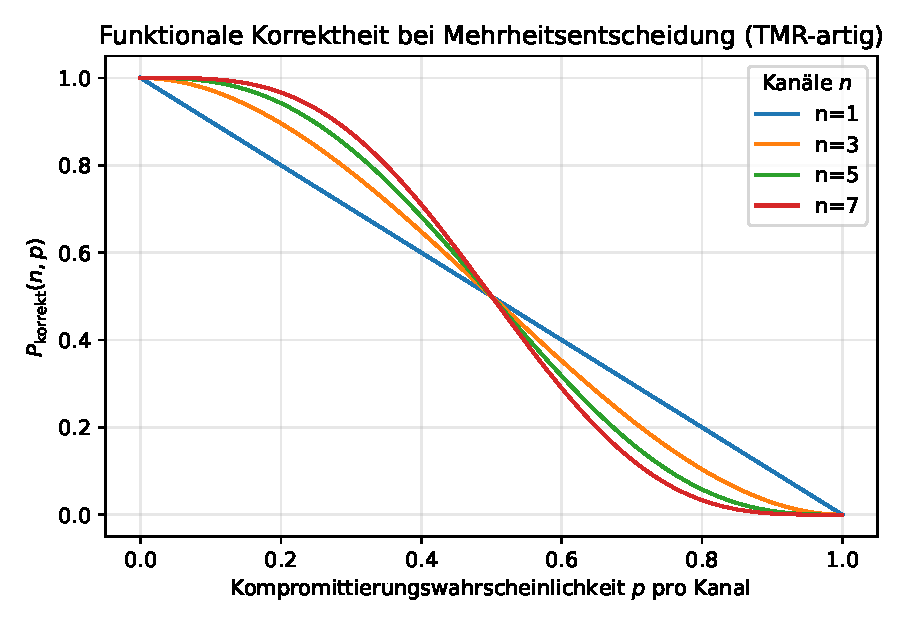
\includegraphics[width=0.85\textwidth]{plot1_korrektheit.pdf}
	\caption{$P_{\mathrm{Safety}}(n,p)$ nach Satz~\ref{satz:pkorrekt} für $n \in \{1,3,5,7\}$ in Abhängigkeit von der Kompromittierungswahrscheinlichkeit $p$ je Kanal. Für $n=1$ (keine Redundanz) fällt die Kurve linear mit $1-p$; bereits ab $n=3$ toleriert das System einen kompromittierten Kanal, ohne dass die Funktion fehlerhaft wird, solange $p$ moderat bleibt. Mit wachsendem $n$ wird die Kurve zunehmend stufenförmig steiler um $p=0{,}5$, in Übereinstimmung mit Lemma~\ref{lem:monotonie} und Lemma~\ref{lem:grenzwert}.}
	\label{fig:korrektheit}
\end{figure}

\begin{figure}[h]
	\centering
	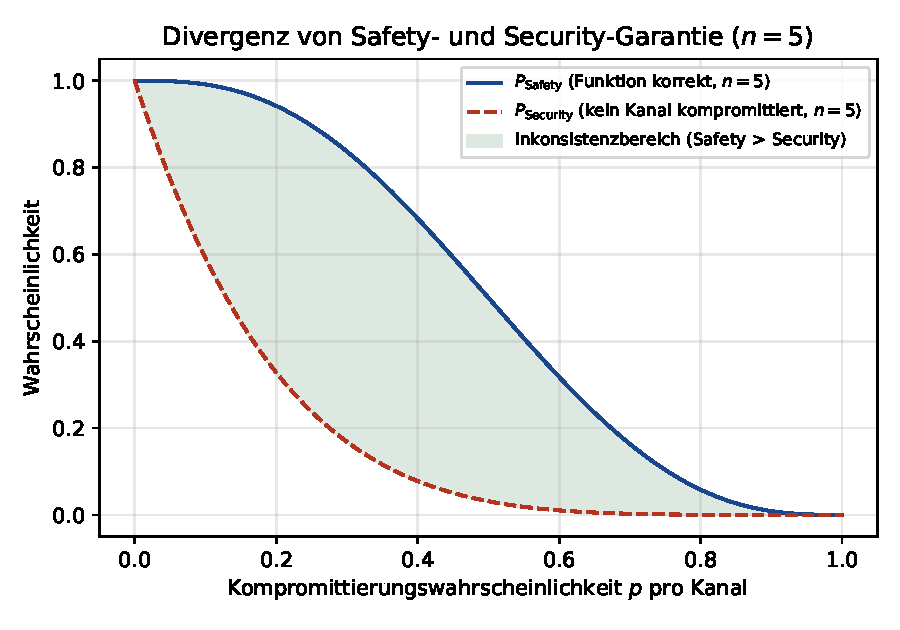
\includegraphics[width=0.85\textwidth]{plot2_divergenz.pdf}
	\caption{Gegenüberstellung von $P_{\mathrm{Safety}}(5,p)$ und $P_{\mathrm{Security}}(5,p)$ gemäß Satz~\ref{satz:pkorrekt} und Satz~\ref{satz:psecure}. Die grün schattierte Fläche markiert den nach Satz~\ref{satz:divergenz} für alle $p \in (0,1)$ nichtleeren Inkonsistenzbereich, in dem die Funktion mit hoher Wahrscheinlichkeit korrekt arbeitet ($S(x)$ wahr), obwohl mindestens ein Kanal mit erheblicher Wahrscheinlichkeit kompromittiert ist ($T(x)$ falsch). Dieser Bereich entspricht exakt dem in Korollar~\ref{kor:inkonsequenz} beschriebenen Szenario: ein erfolgreicher Cyberangriff auf einen Kanal, dessen Wirkung durch den Safety-Mechanismus (Mehrheitsentscheidung) vollständig maskiert wird.}
	\label{fig:divergenz}
\end{figure}

\begin{figure}[h]
	\centering
	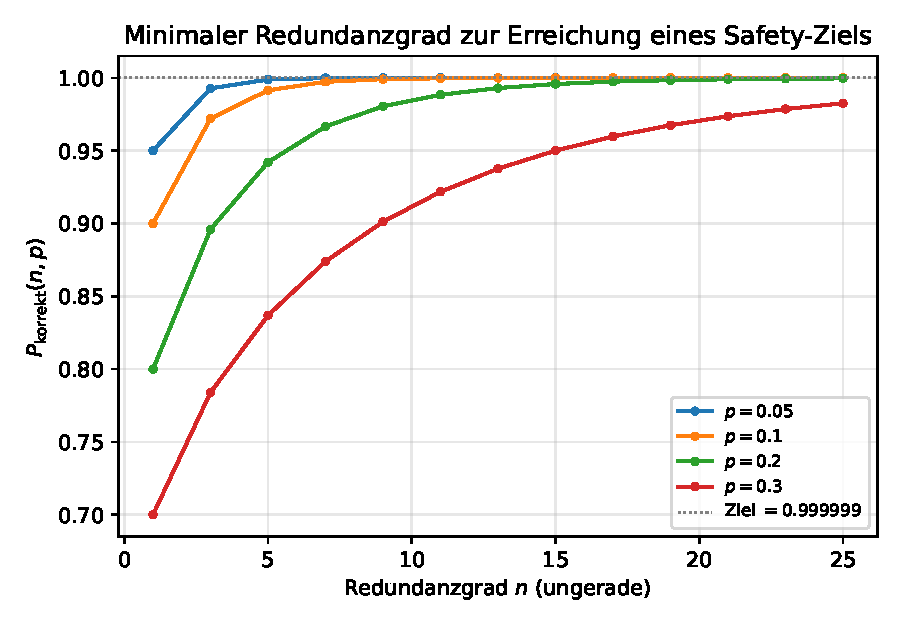
\includegraphics[width=0.85\textwidth]{plot3_redundanzgrad.pdf}
	\caption{Erforderlicher Redundanzgrad $n$, um $P_{\mathrm{Safety}}(n,p)$ über ein Zielniveau von $0{,}999999$ zu heben, für verschiedene Kompromittierungswahrscheinlichkeiten $p \in \{0{,}05,\,0{,}1,\,0{,}2,\,0{,}3\}$. Die Kurven illustrieren Satz~\ref{satz:minimalradundanz}: Je näher $p$ an die kritische Schwelle $0{,}5$ heranrückt, desto stärker wächst der zur Zielerreichung notwendige Redundanzgrad, da die Kullback-Leibler-Divergenz $D(0.5\|p)$ gegen Null geht.}
	\label{fig:redundanzgrad}
\end{figure}

\section{Diskussion}

Die formalen Ergebnisse aus Abschnitt~3 bestätigen die eingangs aufgestellte These: Die getrennte Betrachtung von Safety und Security als unabhängige Zielsysteme ist technisch inkonsequent, da beide Disziplinen auf demselben zugrunde liegenden Mechanismus -- Redundanz mit Mehrheitsentscheidung -- beruhen, jedoch unterschiedliche Schwellenwerte an diesen Mechanismus anlegen. Safety verlangt effektiv nur \emph{Mehrheitsintegrität} ($K \leq \lfloor (n-1)/2 \rfloor$), Security im klassischen Sinne verlangt \emph{Vollintegrität} ($K = 0$). Korollar~\ref{kor:inkonsequenz} zeigt formal, dass ein System in genau dem vom Nutzer beschriebenen Zustand sein kann: ein Safety-Mechanismus greift, die Funktion ist sichergestellt, und dennoch hat ein Cyberangriff das Steuergerät (einen Kanal) bereits manipuliert.

Die praktische Konsequenz ist, dass Audits, Zertifizierungen und Bedrohungsmodelle, die Safety-Cases (ISO~26262) und Security-Cases (ISO/SAE~21434) getrennt führen, regelmäßig zu widersprüchlichen Aussagen über denselben Systemzustand gelangen können. Der in dieser Arbeit vorgeschlagene Begriff der \emph{Redundanzsicherheit} schlägt vor, beide Disziplinen unter dem gemeinsamen Prädikat $S(x)$ zu vereinen und die Ursache der Kanalkompromittierung (zufällig vs.\ vorsätzlich) als orthogonale, aber für die Bewertung der Gesamtsicherheit nachrangige Eigenschaft zu behandeln. Dies bedeutet nicht, dass Security-Maßnahmen wertlos wären -- im Gegenteil, sie reduzieren $p$, also die Kompromittierungswahrscheinlichkeit je Kanal, und wirken damit multiplikativ auf $P_{\mathrm{Safety}}(n,p)$ -- sondern dass die binäre Klassifikation „sicher/unsicher'' stets relativ zu einem expliziten Redundanzmodell und einer expliziten Schwelle (Mehrheits- vs. Vollintegrität) zu erfolgen hat.

\section{Zusammenfassung}

Diese Arbeit zeigt formal, dass Funktionale Sicherheit (Safety) und Cyber Security keine unabhängigen Eigenschaften eines Systems sind, sondern zwei unterschiedliche Schwellenwerte desselben zugrunde liegenden Redundanzmechanismus darstellen. Die zentralen Beiträge sind:

\begin{itemize}
	\item Formaler Nachweis, dass Security (Vollintegrität) Safety (Mehrheitskorrektheit) impliziert, die Umkehrung jedoch nicht gilt (Satz~\ref{satz:implikation}).
	\item Geschlossene Formeln für $P_{\mathrm{Safety}}(n,p)$ und $P_{\mathrm{Security}}(n,p)$ unter dem Bernoulli-Modell unabhängiger Kanalkompromittierung (Satz~\ref{satz:pkorrekt}, Satz~\ref{satz:psecure}).
	\item Beweis der strikten Divergenz beider Größen für jeden nichttrivialen Redundanzgrad $n \geq 3$ (Satz~\ref{satz:divergenz}).
	\item Asymptotisches Grenzverhalten: Safety konvergiert mit wachsendem $n$ gegen Gewissheit, Security gegen Null (Lemma~\ref{lem:grenzwert}).
	\item Eine Chernoff-basierte hinreichende Bedingung für den minimal notwendigen Redundanzgrad zur Erreichung eines Safety-Ziels (Satz~\ref{satz:minimalradundanz}).
\end{itemize}

\subsection{Anwendungen}

Das vorgestellte Modell eignet sich insbesondere für:
\begin{itemize}
	\item Quantitative Bewertung von Steuergeräte-Architekturen mit Lockstep- oder TMR-Redundanz hinsichtlich kombinierter Safety-/Security-Risiken.
	\item Auslegung des Redundanzgrades $n$ in sicherheitskritischen Architekturen unter expliziter Berücksichtigung einer Angreifer-induzierten Kompromittierungswahrscheinlichkeit $p$.
	\item Vereinheitlichte Bedrohungs- und Gefährdungsanalysen, die Safety-Cases (ISO~26262) und Security-Cases (ISO/SAE~21434) auf ein gemeinsames probabilistisches Modell zurückführen.
	\item Bewertung der Wirksamkeit von Security-Maßnahmen (Reduktion von $p$) im Vergleich zur Erhöhung des Redundanzgrades $n$ als alternative oder komplementäre Strategie.
	\item Audit- und Zertifizierungsprozesse, in denen die in Korollar~\ref{kor:inkonsequenz} beschriebene Inkonsequenz explizit dokumentiert und durch ein gemeinsames Prädikat $S(x)$ ersetzt werden soll.
\end{itemize}

\subsection{Ausblick}

Die in dieser Arbeit entwickelte Theorie der Redundanzsicherheit eröffnet eine Reihe weiterführender Forschungsrichtungen, die im Folgenden ausführlich diskutiert werden.

\textbf{1. Abschwächung der Unabhängigkeitsannahme (A1).} Das vorliegende Modell setzt voraus, dass die Kompromittierungsereignisse $K_i(x)$ der einzelnen Kanäle stochastisch unabhängig sind. In realen Architekturen ist diese Annahme insbesondere bei Cyberangriffen häufig verletzt, da ein erfolgreicher Angriff auf einen gemeinsamen Bus, ein gemeinsames Betriebssystem oder eine gemeinsame Kryptobibliothek mehrere Kanäle gleichzeitig kompromittieren kann (sogenannte \emph{Common-Cause-Angriffe}, das Security-Analogon zum klassischen Common-Cause-Failure der Safety-Literatur). Eine naheliegende Erweiterung besteht darin, $K_i(x)$ als korrelierte Zufallsvariablen über ein Copula-Modell oder ein Faktor-Modell mit gemeinsamer latenter Angriffsvariablen zu beschreiben und die in Satz~\ref{satz:pkorrekt} und Satz~\ref{satz:psecure} hergeleiteten geschlossenen Formeln entsprechend zu verallgemeinern. Insbesondere wäre zu untersuchen, ob und unter welchen Korrelationsstrukturen die in Satz~\ref{satz:divergenz} bewiesene strikte Divergenz erhalten bleibt oder ob es Korrelationsregime gibt, in denen $P_{\mathrm{Safety}}$ und $P_{\mathrm{Security}}$ konvergieren.

\textbf{2. Adaptive und strategische Angreifermodelle.} Das vorliegende Modell behandelt $p$ als exogenen, vom Angreifer unabhängig pro Kanal angewendeten Parameter. In der Security-Literatur ist es jedoch üblich, einen rationalen Angreifer zu modellieren, der gezielt eine minimale Anzahl von $\lceil n/2 \rceil$ Kanälen angreift, um die Mehrheitsentscheidung gezielt zu kippen, anstatt Kanäle zufällig und unabhängig zu kompromittieren. Eine spieltheoretische Erweiterung des Modells, in der ein Angreifer mit begrenztem Budget $B$ wählt, welche und wie viele Kanäle er angreift, und ein Verteidiger den Redundanzgrad $n$ sowie die Diversität der Kanäle (unterschiedliche Hardware, unterschiedliche Software-Implementierungen) als Gegenmaßnahme wählt, würde das Modell von einer rein probabilistischen zu einer spieltheoretischen Sicherheitsanalyse weiterentwickeln. Insbesondere ist die Frage von Interesse, ab welchem Diversitätsgrad ein gezielter Angriff auf $\lceil n/2\rceil$ Kanäle ökonomisch unattraktiv gegenüber einem ungezielten Angriff wird.

\textbf{3. Dynamische und zeitabhängige Systeme.} Das vorliegende Modell betrachtet eine einzelne Eingabe $x$ zu einem festen Zeitpunkt. Reale Steuergeräte verarbeiten jedoch kontinuierliche Eingabeströme über die Zeit, wobei ein Angreifer einen Kanal über mehrere Zyklen hinweg schrittweise kompromittieren kann (z.\,B. durch sukzessive Manipulation von Kalibrierdaten). Eine zeitdiskrete Markov-Erweiterung des Modells, in der der Kompromittierungszustand jedes Kanals einem Markov-Prozess mit Übergangswahrscheinlichkeiten für Kompromittierung und Wiederherstellung (z.\,B. durch Neustart, Re-Flashing oder Watchdog-Mechanismen) folgt, würde die Analyse auf realistische Betriebsszenarien mit Langzeitverhalten erweitern. Von besonderem Interesse wäre die Herleitung einer stationären Verteilung für $P_{\mathrm{Safety}}(n,p,t)$ und die Bestimmung der minimalen Wiederherstellungsrate, die erforderlich ist, um trotz fortlaufender Angriffsversuche eine langfristig stabile Safety-Garantie aufrechtzuerhalten.

\textbf{4. Heterogene Voter-Architekturen.} Das vorliegende Modell beschränkt sich auf den einfachen Mehrheits-Voter $V_n$. In der Praxis kommen komplexere Entscheidungsarchitekturen zum Einsatz, etwa gewichtete Voter (bei denen vertrauenswürdigeren Kanälen mehr Gewicht zukommt), hierarchische Voter-Bäume oder byzantinische Fehlertoleranzprotokolle, die explizit für die Anwesenheit eines aktiv täuschenden (nicht nur ausfallenden) Kanals ausgelegt sind. Eine Übertragung der hier entwickelten Safety-/Security-Divergenzanalyse auf das byzantinische Fehlermodell, in dem ein kompromittierter Kanal nicht nur einen falschen, sondern einen adaptiv gewählten, bestmöglich täuschenden Wert ausgeben kann, ist eine naheliegende und praktisch bedeutsame Erweiterung; insbesondere die bekannte Schranke $n \geq 3f+1$ zur Toleranz von $f$ byzantinischen Fehlern (vgl.\ \cite{lamport1982}) ließe sich direkt mit der hier definierten Größe $P_{\mathrm{Security}}(n,p)$ in Beziehung setzen.

\textbf{5. Empirische Validierung an realen Steuergeräte-Architekturen.} Die in dieser Arbeit hergeleiteten Formeln beruhen auf einem abstrakten Bernoulli-Modell. Eine wichtige Folgearbeit besteht in der empirischen Schätzung von $p$ für reale Fahrzeugarchitekturen, etwa auf Basis historischer Felddaten zu Hardwarefehlern (für die Safety-Komponente von $p$) und auf Basis von Penetrationstests sowie veröffentlichten Schwachstellendatenbanken wie der CVE-Datenbank (für die Security-Komponente von $p$). Eine solche empirische Kalibrierung würde es erlauben, die in Satz~\ref{satz:minimalradundanz} hergeleitete Mindestredundanz für konkrete Steuergeräte-Typen (z.\,B. Bremssteuergeräte, Lenkungssteuergeräte) numerisch zu bestimmen und mit den in der Praxis tatsächlich verbauten Redundanzgraden zu vergleichen.

\textbf{6. Verbindung zum Subgraph Algorithmus.} Da Kanäle in modernen Steuergeräten häufig durch unterschiedliche, aber funktional äquivalente Software-Implementierungen realisiert werden (Diversität als Schutz gegen korrelierte Software-Fehler und gemeinsame Angriffsvektoren), stellt sich die Frage, wie strukturelle Ähnlichkeit zwischen den Kontrollflussgraphen bzw. Abstract Syntax Trees zweier Kanal-Implementierungen quantifiziert werden kann, um eine zu geringe Diversität (und damit ein erhöhtes Korrelationsrisiko im Sinne von Punkt~1 dieses Ausblicks) frühzeitig zu erkennen. Der in einer vorangegangenen Arbeit entwickelte Subgraph Algorithmus mit Laufzeit $\Theta(n^3)$ (vgl.\ \texttt{github.com/hjstephan86/subgraph}) liefert hierfür einen naheliegenden Ausgangspunkt: Zwei Kanal-Implementierungen mit hoher struktureller Subgraph-Ähnlichkeit ihrer AST-Repräsentationen wären als Kandidaten für korrelierte, gemeinsam ausnutzbare Schwachstellen zu kennzeichnen, während eine geringe strukturelle Ähnlichkeit auf eine für die Unabhängigkeitsannahme A1 günstige echte Diversität hindeutet. Die Entwicklung eines kombinierten Maßes aus struktureller Subgraph-Distanz und der hier definierten Redundanzsicherheit $P_{\mathrm{Safety}}(n,p)$ wird als vielversprechende Verbindung beider Forschungslinien für zukünftige Arbeiten vorgeschlagen.

\textbf{7. Normative und regulatorische Implikationen.} Schließlich wirft diese Arbeit die Frage auf, ob die organisatorische Trennung von Safety- und Security-Nachweisen in aktuellen Normen (ISO~26262 für Safety, ISO/SAE~21434 für Security) durch ein gemeinsames, redundanzbasiertes Nachweisverfahren ergänzt oder ersetzt werden sollte, das explizit das hier bewiesene Inkonsistenzphänomen (Korollar~\ref{kor:inkonsequenz}) adressiert. Eine interdisziplinäre Weiterentwicklung dieser Arbeit in Richtung eines kombinierten „Redundanzsicherheits-Case'' als Ergänzung zu den etablierten Safety- und Security-Cases erscheint sowohl wissenschaftlich als auch praktisch lohnend.

\subsection{Implementierungshinweis}

Die in Abschnitt~4 verwendeten numerischen Berechnungen und Diagramme wurden mit Python und \texttt{matplotlib} erstellt; Quellcode und weiterführende Arbeiten sind verfügbar unter: \url{https://github.com/hjstephan86/science}.

\begin{thebibliography}{9}

\bibitem{iso26262}
International Organization for Standardization.
\emph{ISO 26262: Road vehicles -- Functional safety}.
ISO, Genf, 2018.

\bibitem{iso21434}
International Organization for Standardization / SAE International.
\emph{ISO/SAE 21434: Road vehicles -- Cybersecurity engineering}.
ISO/SAE, 2021.

\bibitem{lamport1982}
Lamport, L., Shostak, R., Pease, M.
\emph{The Byzantine Generals Problem}.
ACM Transactions on Programming Languages and Systems, 4(3), S.~382--401, 1982.

\bibitem{condorcet1785}
de Condorcet, N.
\emph{Essai sur l'application de l'analyse à la probabilité des décisions rendues à la pluralité des voix}.
Imprimerie Royale, Paris, 1785.

\bibitem{chernoff1952}
Chernoff, H.
\emph{A Measure of Asymptotic Efficiency for Tests of a Hypothesis Based on the Sum of Observations}.
Annals of Mathematical Statistics, 23(4), S.~493--507, 1952.

\bibitem{avizienis2004}
Avižienis, A., Laprie, J.-C., Randell, B., Landwehr, C.
\emph{Basic Concepts and Taxonomy of Dependable and Secure Computing}.
IEEE Transactions on Dependable and Secure Computing, 1(1), S.~11--33, 2004.

\bibitem{epp2026subgraph}
Epp, S.
\emph{Der Subgraph Algorithmus}.
github.com/hjstephan86/subgraph, 2026.

\end{thebibliography}

\end{document}

